% !TEX root = ../Dokumentation.tex
\section{Technologierecherche}
\subsection{Funktionsweise der Hardware}
Für die geplante Arbeit wird ein Raspberry Pi 3, eine 32GB SD-Karte, eine Basisplatine, Sensorplatinen mit Temperaturfühlern sowie entsprechende Verbindungskabel verwendet. Das Raspberry Pi ist ein Einplatinencomputer und eignet sich mit seinen Funktionen und Komponenten besonders gut für diese Arbeit. Über die elektrischen Anschlusspunkte, auch GPIOs genannt, werden die Messsignale des Temperatursensors abgefragt. Mittels der Basisplatine, welche an das Raspberry angeschlossen wird, können die gelieferten Daten der angeschlossenen Sensoren von einem analogen zu einem digitalen Signalen umgewandelt werden.
Diese digitalen Signale können so in Temperaturwerte umgerechnet und für eine kontinuierliche Anzeige bereitgestellt werden.

\begin{figure}[H]%Position festigen
\centering
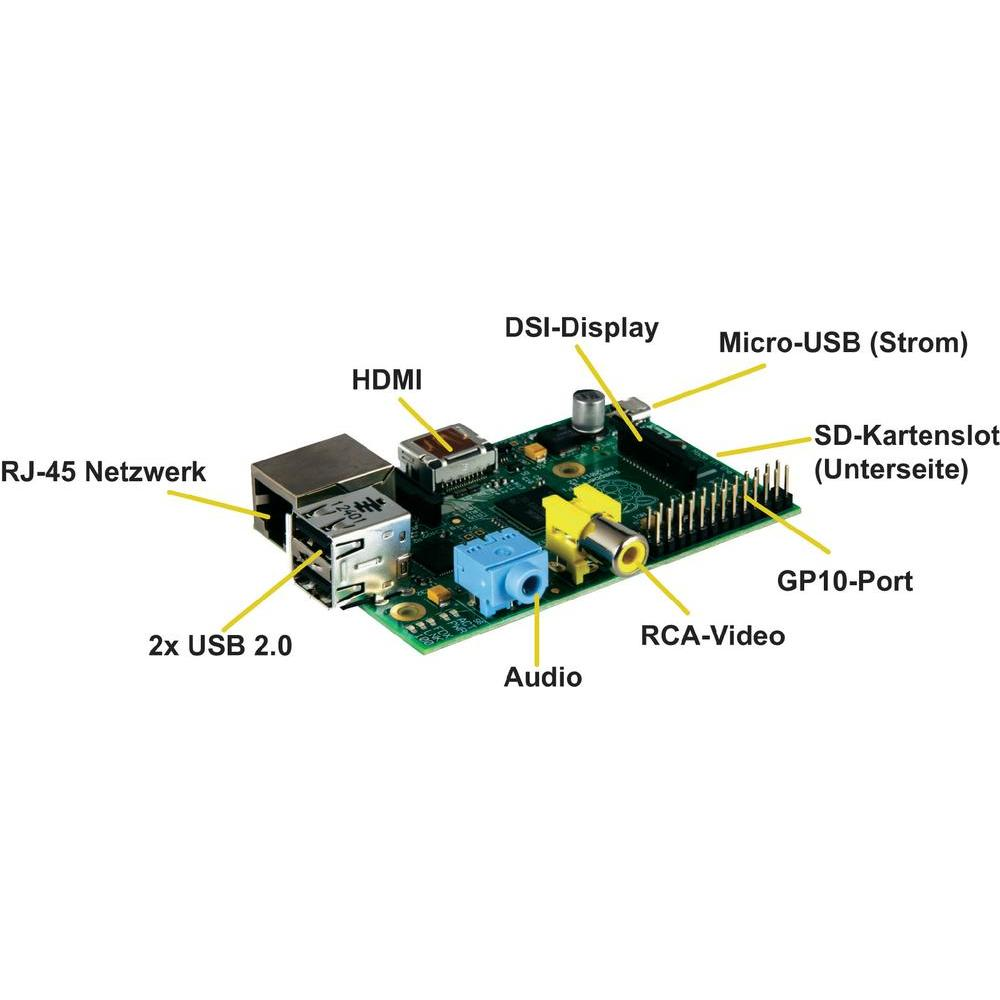
\includegraphics[width=1\textwidth]{Images/RaspberryPi.jpg}
\caption{Pi (Quelle www.Conrad.ch)}
\label{fig:raspi}
\end{figure}

\subsubsection{GPIO}
General-purpose input/output (GPIO) ist ein digitaler Anschlusspunkt, welcher vom RaspberryPi zur Verfügung gestellt wird. Über diese Schnittstelle können die Werte der anschlossenen Sensoren übertragen werden. Für die Auswertung analoger Sensoren muss entsprechend ein Analog- Digitalwandler verwendet werden.

\subsubsection{Sensortypen}
<tbd>

\subsection{Software Entwurfsmuster}
Die Software für die Temperaturüberwachung muss, aufgrund des Dauerbetriebes, robust, energieschonend und erweiterbar gestaltet werden. Um diese Anforderungen zu erreichen, haben wir einige Entwurfsmuster verwendet.\\
Der Zugriff auf die Sensorwerte soll mittels Singleton-Pattern realisiert werden, damit keine parallele Zugriffe erfolgen, wenn keine notwendig sind. Ebenso soll dieses Pattern für die Ausgabe der Log-Meldungen zum Einsatz kommen.\\
Die Sensoren müssen nicht im Dauerlauf abgefragt werden, da sich die Temperatur selten im Sekundentakt ändert. Deshalb sollen die Sensoren alle fünf bis zehn Sekunden ihre Werte rapportieren und nicht gepollt werden. Erreicht soll diese Anforderung mit dem Observer-Pattern.\\
Um eine regelmässige Prüfung der Sensoren sicherzustellen, wird ein Watchdog erstellt, welcher regelmässig über alle Kanäle iteriert und aktive, sowie inaktive Sensoren meldet. Werden neue Sensoren registriert, soll wür jeden Sensor ein Thread gestartet werden. Fällt ein Sensor aus, oder wird entfernt, wird der entsprechende Thread gestoppt.\\
Für die Anzeige der Sensordaten für die Webansicht, werden die Sensordaten in einer XML-Datei verwendet werden, welche mittels Pugixml\footnote{Pugixml ist ein leichtgewichtiger, open Source XML-Parser. www.pugixml.org} gelesen und verändert werden kann. Die gleiche XML-Datei soll für alle benötigten Kofigurationen verwendet werden.\\
Basierend auf den Erfahrungen des Teams, soll die Software in C++ realisiert werden.
